% !TEX encoding = UTF-8 Unicode

\documentclass[a4paper]{article}

\usepackage{color}
\usepackage{xcolor}
\usepackage{url}
\usepackage[T2A]{fontenc} % enable Cyrillic fonts
\usepackage[utf8]{inputenc} % make weird characters work
\usepackage{graphicx}
\usepackage{amsthm}
\usepackage{amsmath}
\usepackage{booktabs,hhline}

\usepackage{multirow}       % used for making multirow tables (Nemanja)
\usepackage{minted}

%\usepackage[english,serbian]{babel}
\usepackage[english,serbianc]{babel} %ukljuciti babel sa ovim opcijama, umesto gornjim, ukoliko se koristi cirilica

\usepackage[unicode]{hyperref}
\hypersetup{colorlinks,citecolor=green,filecolor=green,linkcolor=blue,urlcolor=blue}

\newtheorem{primer}{Пример}[section] %ćirilični primer
%\newtheorem{primer}{Primer}[section]

\newtheorem{definic}{Дефиниција}
\newcommand{\norm}[1]{\left\lVert#1\right\rVert}

\begin{document}

%TODO smisliti naslov
\title{Google DeepDream \\ \small{Семинарски рад у оквиру курса\\Истраживање података\\ Математички факултет}}

\author{Немања Мићовић\\ nmicovic@outlook.com}
\date{}
\maketitle

\abstract{
    Dodati posle.
}

\tableofcontents

\newpage

% ---------------------------------------------------------------------------------------------------------------------
\section{Увод}
% ---------------------------------------------------------------------------------------------------------------------
Неуронске мреже данас постижу изузетне резултате на многим пољима вештачке интелигенције.
Artificial Neural Networks have spurred remarkable recent progress in image classification and speech recognition.
But even though these are very useful tools based on well-known mathematical methods,
we actually understand surprisingly little of why certain models work and others don’t.
So let’s take a look at some simple techniques for peeking inside these networks.

% ---------------------------------------------------------------------------------------------------------------------
\section{Неуронске мреже}
% ---------------------------------------------------------------------------------------------------------------------

% ---------------------------------------------------------------------------------------------------------------------
\subsection{Перцептрон}
% ---------------------------------------------------------------------------------------------------------------------
% TODO
Слика \ref{fig:perceptron} приказује перцептрон.

\begin{figure}[h!]
\begin{center}
    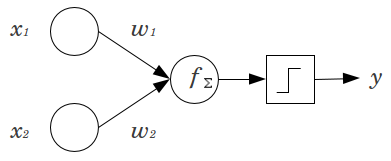
\includegraphics[scale=0.5]{./resources/perceptron.png}
\end{center}
\caption{Пецептрон}
\label{fig:perceptron}
\end{figure}


% ---------------------------------------------------------------------------------------------------------------------
\subsection{Конволутивне неуронске мреже}
% ---------------------------------------------------------------------------------------------------------------------
Идеја о конволутивним неуронским мрежама јавила се још раних деведесетих \cite{covnetBirth},
но праву популарност конволутивне мреже достижу у последњих неколико година услед могућности
да се процес тренинга мрежа ефикасно паралелизује на графичким картицама. Успешна паралелизација
је омогућила да се врши тренинг над милијардама података као и да се користe дубоке неуронске мреже
са по неколико хиљада слојева. Популарност конволутивних мрежа нагло пораста, а сама тема постаје
изузетно истраживачки популарна.

Конволутивне неуронске мреже постигле су изузетне резултате у проблемима попут класификације \cite{NIPS2012_4824,
ciregan, DBLP:journals/corr/SimonyanZ14a},
а генерално се могу користити када је у питању нека врста улазног сигнала (слика, звук, видео). Коришћене су и
за класификацију текста \cite{cnnForText} а занимљива је и примена у раду \cite{cnnForAutism}.

Конволутивне мреже се могу применити на било какве податке који поседују структуралну информацију.
Другачије речено, уколико се редослед података/сигнала једне инстанце пермутује, губи се суштина информације.
На пример, уколико се пермутују пиксели слике, губи се информација као и сам објекат који је на слици.

Неурони конволутивне мреже уче да препознају неку врсту шаблона на основу тренинг скупа. Што је неурон дубље у мрежи,
шаблон који препознаје постаје комплекснији. На примеру слике и препознавању лица,
један од неурона у почетним слојевима би препознавао хоризонталну линију, а неурон при крају мреже, очи или нос. Комбинација неурона
омогућава да се дође до одговора шта је на слици. Често се на крају користи софтмакс техника како би се
неурони на последњем слоју користили за оцену вероватноће класе којој инстанца припада.

Слика \ref{fig:cnn} приказује пример конволутивне мреже. У делу \ref{subsec:arch} ће детаљније бити образложени делови типичне архитектуре.

\begin{figure}[h!]
\begin{center}
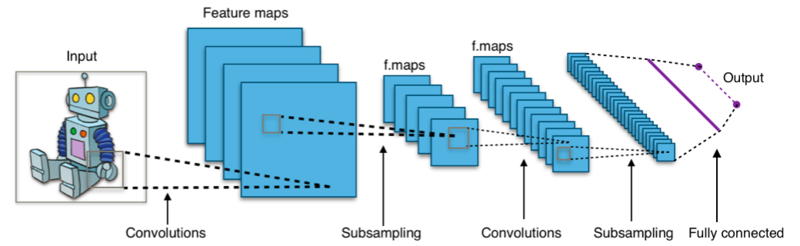
\includegraphics[width=\textwidth]{resources/typical-cnn.png}
\end{center}
\caption{Пример архитектуре конволутивне неуронске мреже}
\label{fig:cnn}
\end{figure}

\subsubsection{ILSVRC}
Најпознатији скуп података у области класификације слика је \textit{ImageNet} који се
користи на такмичењу \textit{ILSVRC}. \textit{ImageNet} за циљ има да понуди барем 1000 слика
за сваки скуп синонима у бази \textit{WordNet} којих има преко 100 000.

Google је 2010. године организовао такмичење \textit{The ImageNet Large Scale Visual Recognition Challenge (ILSVRC)}
чија је тема била класификација и препознавање објеката на сликама. Такмичење је за циљ имало да мотивише истраживаче
да даље развијају алгоритме за класификацију објеката на сликама као и да им омогући да своје резултате
могу да упоредe са другима у области. Такмичење се оджава сваке године почевши од 2010. и представља један од
најбитнијих догађаја у овом делу области машинског учења.

Oко 2011. године, грешка класификације на такмичењу је била 25\%, 2012. године је дубока
неуронска мрежа постигла 16\%, а у следећих неколико година је грешка je драстично падала. Слика \ref{fig:imgneterror}
приказује грешку класификације на неколико узастопних такмичења. Занимљиво је приметити да је на
скупу инстанци \textit{ImageNet} конволутивна мрежа постигла нижу грешку класификације од човека.

\begin{figure}[h!]
\begin{center}
    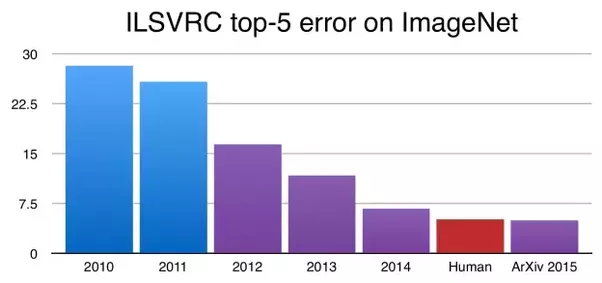
\includegraphics[width=\textwidth]{resources/ilsvrc.png}
\end{center}
\caption{Грешка класификације на скупу \textit{ImageNet}}
\label{fig:imgneterror}
\end{figure}


\subsection{Архитектура конволутивне мреже}
Архитектура конволутивне мреже се састоји из слојева као и код стандардних неуронских мрежа.
Слојеви могу бити:
\begin{itemize}
	\item Потпуно повезани (eng. \textit{fully connected})
	\item Конволутивни (eng. \textit{convolutive})
	\item Пулинг (eng. \textit{pooling})
\end{itemize}

Сликe \ref{fig:nn} и \ref{fig:cnn} приказују разлику између обичне неуронске мреже и конволутивне неуронске мреже.

\label{subsec:arch}

\begin{figure}[!tbp]
	\centering
	\begin{minipage}[b]{0.45\textwidth}
		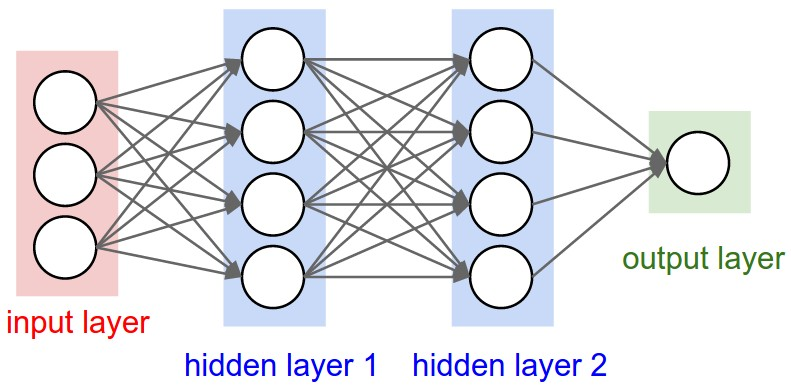
\includegraphics[width=\textwidth]{resources/neural_net}
		\caption{Неуронска мрежа}
		\label{fig:nn}
	\end{minipage}
	\hfill
	\begin{minipage}[b]{0.45\textwidth}
		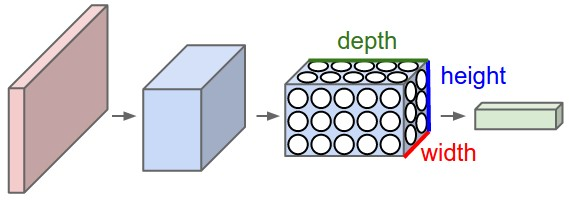
\includegraphics[width=\textwidth]{resources/cnn}
		\caption{Конволутивна неуронска мрежа}
		\label{fig:cnn}
	\end{minipage}
\end{figure}

\subsubsection{Конволуција}

Слика \ref{fig:filters} приказује филтере које је научила мрежа коришћена у раду \cite{NIPS2012_4824}.

\begin{figure}[h!]
\begin{center}
    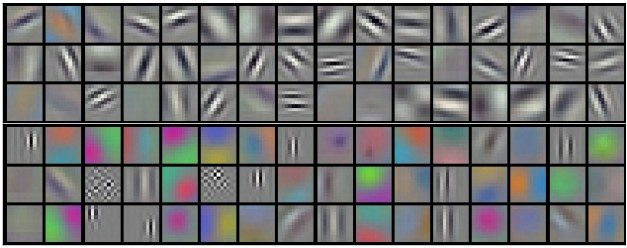
\includegraphics[width=\textwidth]{./resources/filters}
\end{center}
\caption{Пример филтера које је научила конволутивна мрежа}
\label{fig:filters}
\end{figure}

\subsubsection{Pooling}
\subsubsection{Активациона функција}

\subsection{Визуелизација конволутивне мреже}

% ---------------------------------------------------------------------------------------------------------------------
\section{Google Deep dream}
% ---------------------------------------------------------------------------------------------------------------------
\texttt{DeepDream} представља пројекат који је конструисао Google. Главна мотивација за пројекат било је
интересовање истраживача да разумеју и визуализују како се понашају неурони утрениране конволутивне
мреже. 

Приступ који се користи је да се утренираној конволутивној неуронској мрежи којa препознаје слике
проследи нека произвољна слика, а онда се прослеђена слика мења тако да што више активира циљани
слој неуронске мреже. Део \ref{subsec:deepdreamGenerate} ће прецизније изложити процес генерисања слике.

Процес генерисања слике истраживачки тим је називао \textit{сањање} (eng. \textit{dreaming}),
и једна од инспирација су им били снови. Добијене слике поседују халуциногени ефекат који
многе подсећа на снове. Слике \ref{fig:deepdream1} и \ref{fig:deepdream2} приказују неке од добијених слика.

\begin{figure}[h!]
\begin{center}
    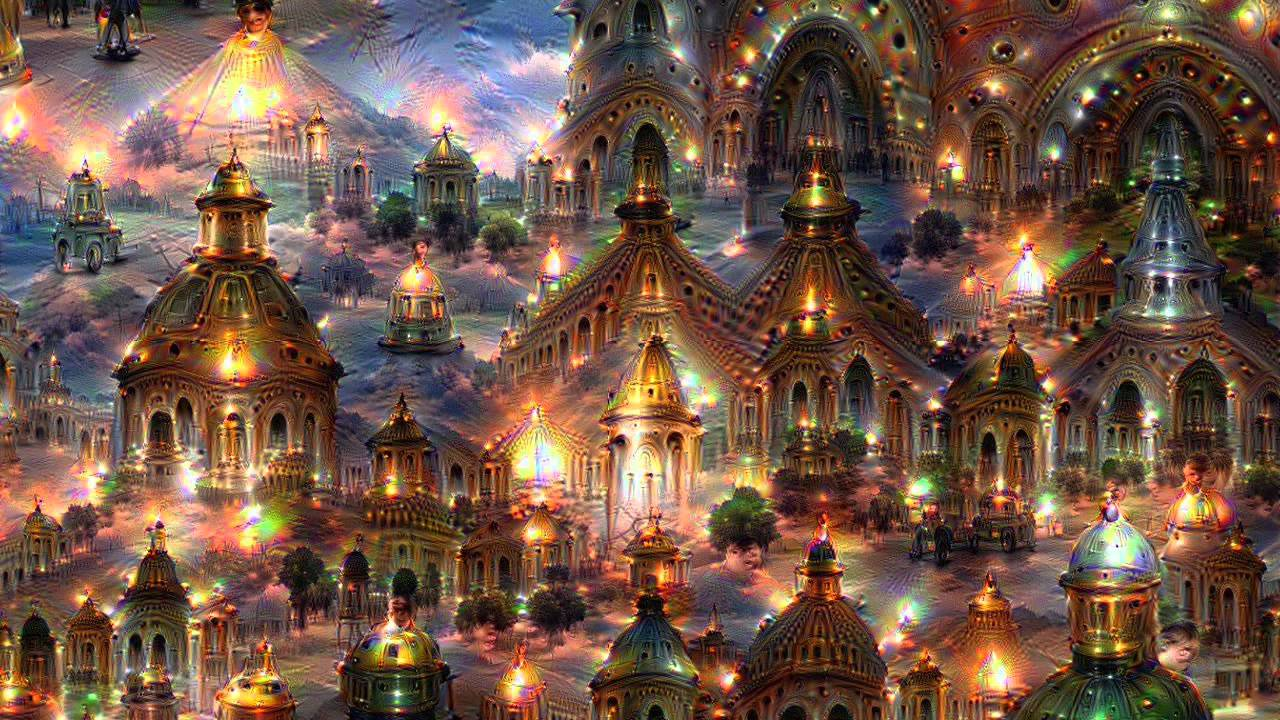
\includegraphics[width=\textwidth]{./resources/deepdream1.jpg}
\end{center}
\caption{Пример слике пројекта \texttt{DeepDream}}
\label{fig:deepdream1}
\end{figure}

\begin{figure}[h!]
\begin{center}
    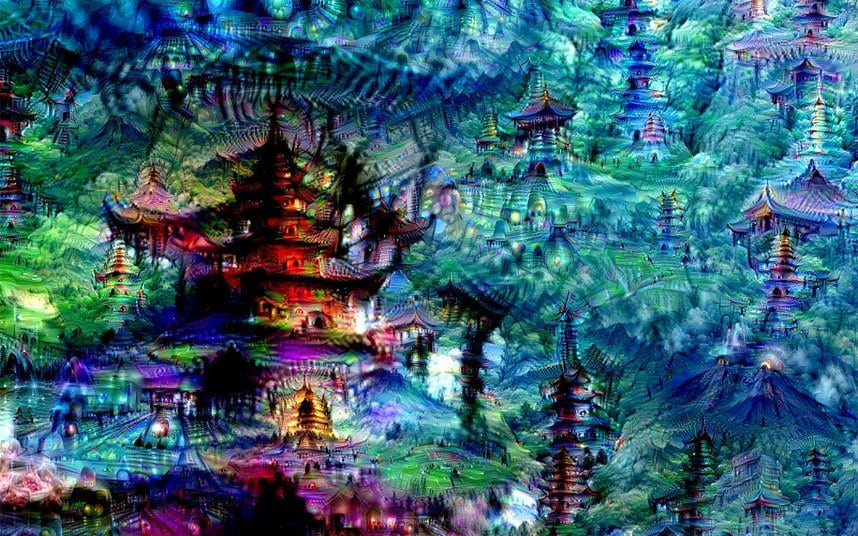
\includegraphics[width=\textwidth]{./resources/deepdream2.jpg}
\end{center}
\caption{Пример слике пројекта \texttt{DeepDream}}
\label{fig:deepdream2}
\end{figure}

\subsection{Генерисање слика}
\label{subsec:deepdreamGenerate}
Реч сан (eng. \textit{dream})
се налази у називу јер је истраживаче ово подсећало на визуелизацију снова. Google је на неки реч
брендирао реч \textit{сањати} (eng. \textit{dream}) у овом контексту и њена употреба је честа када
се мисли на процес генерисања слика које проузрокују тражене активације у тренираној мрежи.

\section{DeepDream генерисање слике - Python}
У овом делу биће приказани делови кода који је коришћен у пројекту \textit{DeepDream}.
Оригинални код доступан је на адреси: \\
\url{https://github.com/google/deepdream}.

\begin{minted}{python}
\end{minted}

% ---------------------------------------------------------------------------------------------------------------------
\section{Закључак}
% ---------------------------------------------------------------------------------------------------------------------
Zakljucak...

\addcontentsline{toc}{section}{Literatura}
\appendix
\bibliography{literature}
\bibliographystyle{plain}


\end{document}
